% Created 2019-05-17 vie 00:13
% Intended LaTeX compiler: pdflatex
\documentclass[11pt]{article}
\usepackage[utf8]{inputenc}
\usepackage[T1]{fontenc}
\usepackage{graphicx}
\usepackage{grffile}
\usepackage{longtable}
\usepackage{wrapfig}
\usepackage{rotating}
\usepackage[normalem]{ulem}
\usepackage{amsmath}
\usepackage{textcomp}
\usepackage{amssymb}
\usepackage{capt-of}
\usepackage{hyperref}
\author{Marco Centurion}
\date{\today}
\title{Manual de Instalación}
\hypersetup{
 pdfauthor={Marco Centurion},
 pdftitle={Manual de Instalación},
 pdfkeywords={},
 pdfsubject={},
 pdfcreator={Emacs 26.1 (Org mode 9.1.9)}, 
 pdflang={English}}
\begin{document}

\maketitle
\tableofcontents


\section{Descripción}
\label{sec:org17588f2}

El presente documento es un breve manual de uso del software
desarrollado en el marco del proyecto de grado "Ingeniería Dirigida
por Modelos aplicada a la configuración de redes de computadoras".

En el mismo se describirán los pasos para crear un proyecto que
utilice el perfil mdcms, para crear elementos en un modelo haciendo
uso del perfil y finalmente para ejecutar la transformación provista.

\section{Proyecto}
\label{sec:org66c8ddb}

Para crear un proyecto Papyrus que utilice el modelo, el primer paso
es hacer click en "File > New > Proyect":

\begin{center}
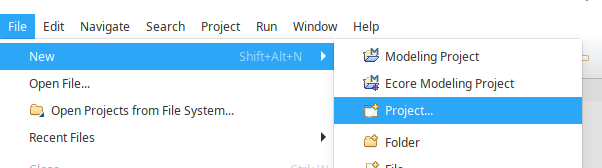
\includegraphics[width=.9\linewidth]{images/proyecto_1.png}
\end{center}

A continuación se debe elegir el tipo de proyecto "Papyrus Project"
dentro de la categoría "Papyrus":

\begin{center}
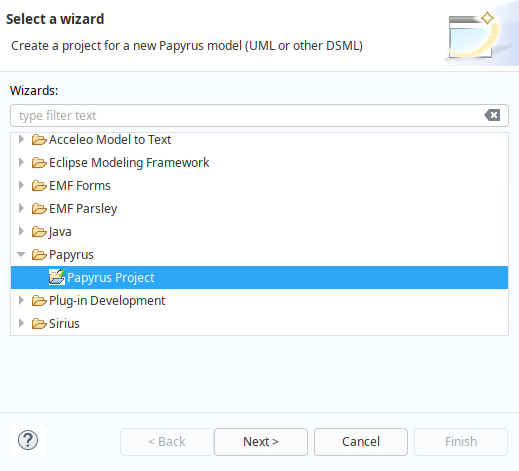
\includegraphics[width=.9\linewidth]{images/proyecto_2.png}
\end{center}

En el siguiente paso dejamos todo como está:

\begin{center}
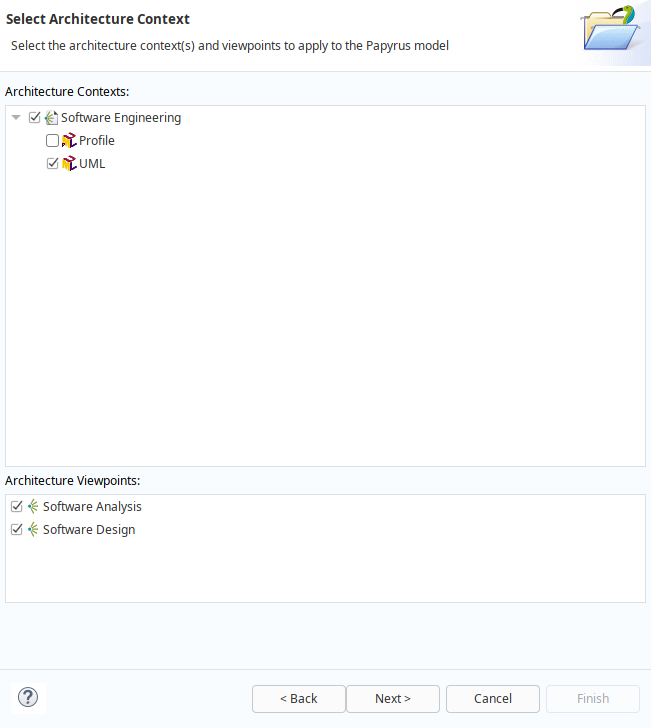
\includegraphics[width=.9\linewidth]{images/proyecto_3.png}
\end{center}

A continuación elegiremos el nombre del proyecto, "Test" en este caso:

\begin{center}
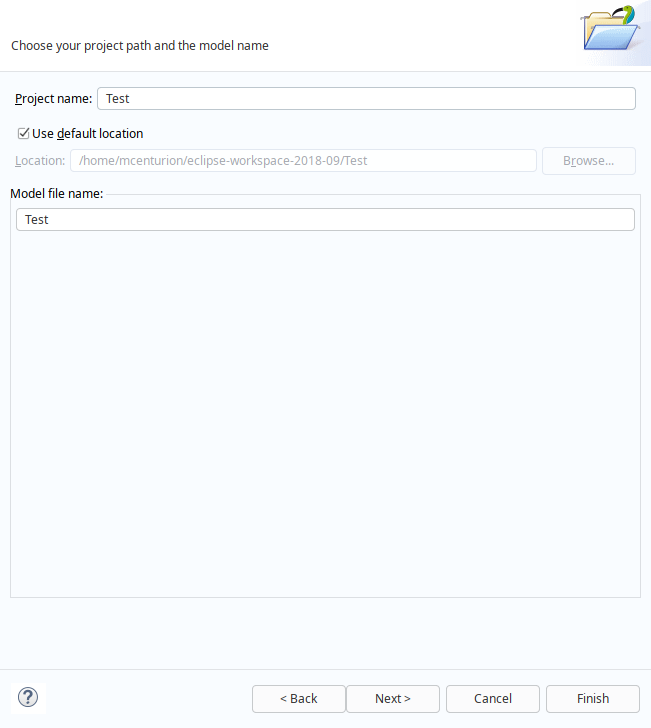
\includegraphics[width=.9\linewidth]{images/proyecto_4.png}
\end{center}

En la siguiente ventana realizaremos dos acciones. Primero
seleccionaremos el tipo de representación "Deployment Diagram":

\begin{center}
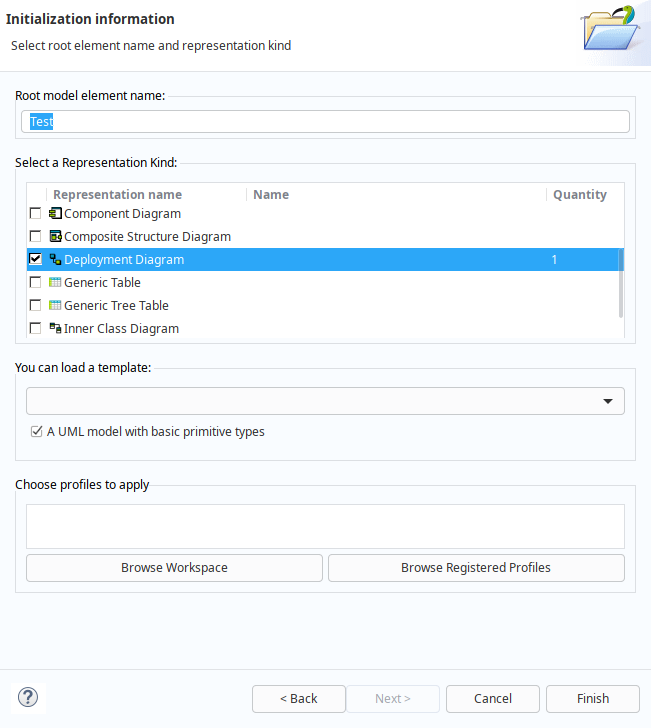
\includegraphics[width=.9\linewidth]{images/proyecto_5.png}
\end{center}

Luego hacemos click en "Browse Registered Profiles" y en la ventana
que aparece eligiremos "MDCMS":

\begin{center}
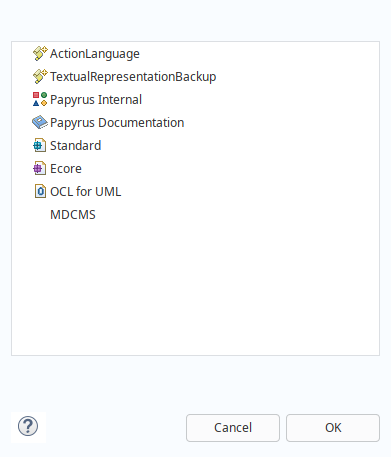
\includegraphics[width=.9\linewidth]{images/proyecto_6.png}
\end{center}

Damos "Finish" y tendremos creado nuestro proyecto.

\section{Modelo}
\label{sec:org056320f}

Una vez creado el proyecto, nos encontraremos con la siguiente
perspectiva:

\begin{center}
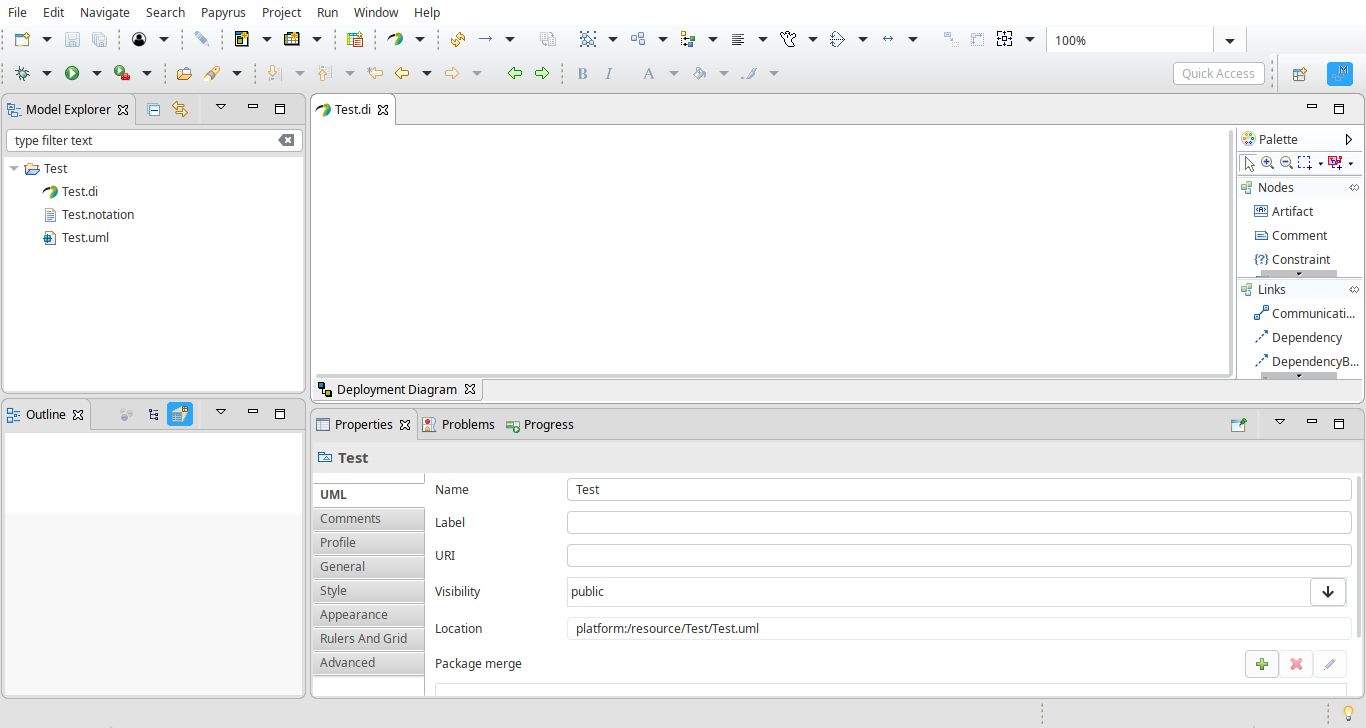
\includegraphics[width=.9\linewidth]{images/modelo_1.png}
\end{center}

De la paleta de la izquierda podremos arrastrar elementos al lienzo
principal. Ahora agregaremos un "Device", ya que queremos representar
un PC:

\begin{center}
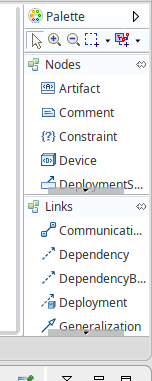
\includegraphics[width=.9\linewidth]{images/modelo_2.png}
\end{center}

Si hacemos click en el elemento creado, en la vista "Properties", en
la pestaña "Profile" podremos hacer click en el boton "+" para agregar
más estereotipos:

\begin{center}
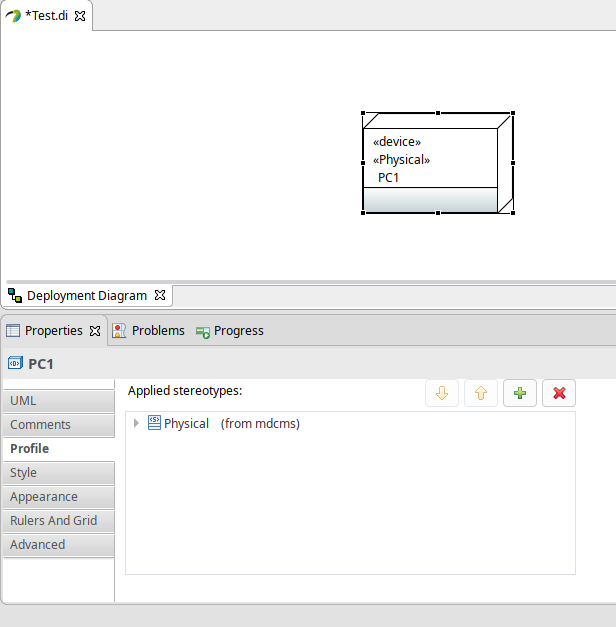
\includegraphics[width=.9\linewidth]{images/modelo_3.png}
\end{center}

Como en este caso queremos representar un PC, en el diálogo que
aparece haremos click en "PC" y en el botón "->", para agregar dicho
estereotipo:

\begin{center}
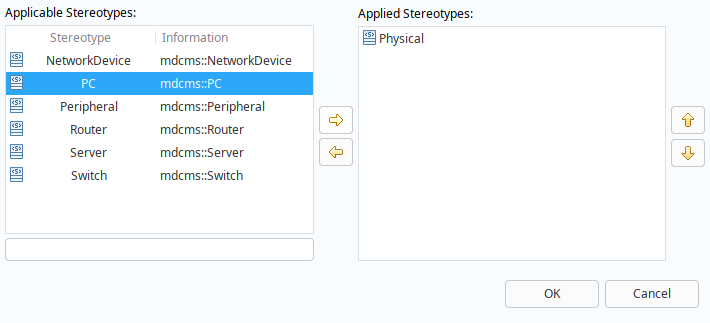
\includegraphics[width=.9\linewidth]{images/modelo_5.png}
\end{center}

Finalmente tenemos representado un PC. Todo lo que resta ahora es, en
la pestaña "Profile", desplegar el estereotipo y completar los
atributos que se presentan:

\begin{center}
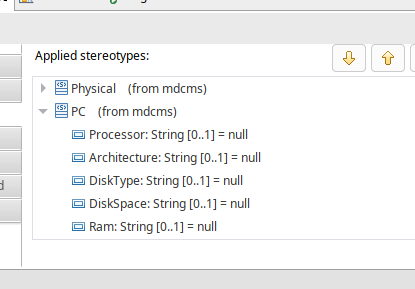
\includegraphics[width=.9\linewidth]{images/modelo_6.png}
\end{center}

\section{Transformación}
\label{sec:org2b6f134}

Una vez tenemos un modelo creado, realizar la transformación para
obtener código puppet es muy sencilla.

En el model explorer debemos ubicar el archivo .uml asociado a nuestro
modelo y hacer click derecho sobre el mismo:

\begin{center}
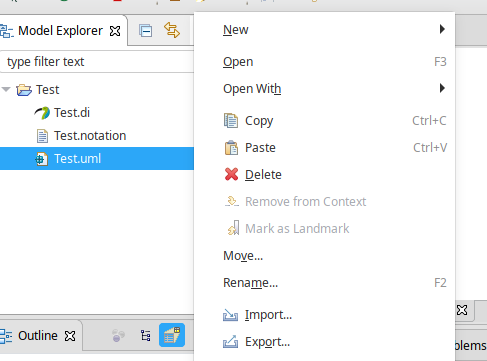
\includegraphics[width=.9\linewidth]{images/transformacion_1.png}
\end{center}

Al final de la lista que se despliega, encontraremos un menú "Acceleo
Model to Text", dentro del cual hay una opción "Generate Mdcm2puppet":

\begin{center}
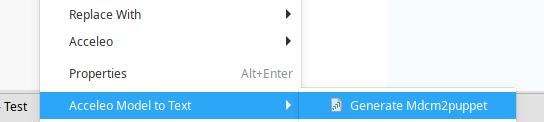
\includegraphics[width=.9\linewidth]{images/transformacion_2.png}
\end{center}

Al hacer click en dicha opción, se llevará a cabo la transformación,
luego de cuya finalización tendremos un directorio "src-gen" con el
código generado:

\begin{center}
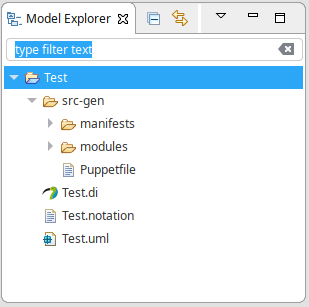
\includegraphics[width=.9\linewidth]{images/transformacion_3.png}
\end{center}
\end{document}